\documentclass[conference]{IEEEtran}
\usepackage{times}

% numbers option provides compact numerical references in the text. 
\usepackage[numbers]{natbib}
\usepackage{multicol}
\usepackage[bookmarks=true]{hyperref}
\usepackage{xcolor}
\usepackage{graphicx}

\pdfinfo{
   /Author (Homer Simpson)
   /Title  (Robots: Our new overlords)
   /CreationDate (D:20101201120000)
   /Subject (Robots)
   /Keywords (Robots;Overlords)
}
\newcommand{\nhatch}[1]{{\leavevmode\color{magenta} Nathan: #1}}

\begin{document}

\title{Curriculum and Imitation Learning for Biped Locomotion on Rough Terrain}

% You will get a Paper-ID when submitting a pdf file to the conference system
\author{Author Names Omitted for Anonymous Review.}

%\author{\authorblockN{Michael Shell}
%\authorblockA{School of Electrical and\\Computer Engineering\\
%Georgia Institute of Technology\\
%Atlanta, Georgia 30332--0250\\
%Email: mshell@ece.gatech.edu}
%\and
%\authorblockN{Homer Simpson}
%\authorblockA{Twentieth Century Fox\\
%Springfield, USA\\
%Email: homer@thesimpsons.com}
%\and
%\authorblockN{James Kirk\\ and Montgomery Scott}
%\authorblockA{Starfleet Academy\\
%San Francisco, California 96678-2391\\
%Telephone: (800) 555--1212\\
%Fax: (888) 555--1212}}


% avoiding spaces at the end of the author lines is not a problem with
% conference papers because we don't use \thanks or \IEEEmembership


% for over three affiliations, or if they all won't fit within the width
% of the page, use this alternative format:
% 
%\author{\authorblockN{Michael Shell\authorrefmark{1},
%Homer Simpson\authorrefmark{2},
%James Kirk\authorrefmark{3}, 
%Montgomery Scott\authorrefmark{3} and
%Eldon Tyrell\authorrefmark{4}}
%\authorblockA{\authorrefmark{1}School of Electrical and Computer Engineering\\
%Georgia Institute of Technology,
%Atlanta, Georgia 30332--0250\\ Email: mshell@ece.gatech.edu}
%\authorblockA{\authorrefmark{2}Twentieth Century Fox, Springfield, USA\\
%Email: homer@thesimpsons.com}
%\authorblockA{\authorrefmark{3}Starfleet Academy, San Francisco, California 96678-2391\\
%Telephone: (800) 555--1212, Fax: (888) 555--1212}
%\authorblockA{\authorrefmark{4}Tyrell Inc., 123 Replicant Street, Los Angeles, California 90210--4321}}


\maketitle

\begin{abstract}
  Biped locomotion with precise foot placement has previously been achieved only for static gaits, using detailed dynamics models and hierarchical optimization-based planning.
  Meanwhile, learning-based approaches to locomotion, such as deep reinforcement learning, are still too sample-inefficient to achieve the precise foot placement necessary to traverse rough terrain.
  In this paper, we improve sample efficiency for learning-based control techniques.
  Our strategy applies to any periodic robotic control task that admits significant prior knowledge.
  First, we engineer a versatile low-level policy (a.k.a. trajectory generator) with interpretable high-level parameters.
  Second, we use reward shaping, imitation learning, and curriculum learning to train a high-level policy for the control task.
  We evaluate this technique with a simulated biped locomotion task over rough terrain.
  To the best of our knowledge, our experiments are the first to achieve such precise foot placement
  using a fast, non-static gait that requires no optimization during policy execution.
\end{abstract}

\IEEEpeerreviewmaketitle


\section{Introduction} \label{sec:intro}

Locomotion is a difficult, underactuated control problem.
\emph{Biped} locomotion is more difficult because the support polygon is small and the center of mass is relatively high.
Biped locomotion on \emph{rough terrain} is more difficult still, because frequent large obstacles make even small mistakes catastrophic.

One way to handle these challenges is with detailed models and extensive optimization.
For example, the WPI-CMU team in the DARPA Robotics Challenge (DRC) controlled ATLAS using a hierarchical optimization approach that carefully controlled the robot's center of mass (CoM) and center of pressure (CoP) \citep{feng2015optimization}.
Such approaches tend to be reliable but slow.
They are physically slow because accurate modeling requires relatively static walking, and also because the optimization procedures are computationally slow.
For the DRC, reliability was more important than speed, but eventually we want to have robots that can traverse rough terrain using faster, dynamic gaits.

Recent advances in reinforcement learning (RL) suggest an alternative approach.
Deep RL is a popular technique to learn highly dynamic motions for humanoids \citep{peng2018deepmimic, heess2017emergence}.
Using sim-to-real techniques, \citet{tan2018sim} have even applied deep RL techniques to physical robots, albeit for quadruped locomotion rather than biped.
The policies learned by deep RL are both computationally and physically fast.
However, due to the extreme sample inefficiency of deep RL algorithms, their effectiveness in more challenging environments---for example, physical bipeds or rough terrain---is uncertain.

One way to address this is to simplify the environment by use of what \citet{iscen2018pmtg} call \emph{policies modulating trajectory generators} (PMTG).
A trajectory generator (TG) is a policy (usually relatively simple) with several high-level parameters.
In environments with a strong prior on what a good policy might look like (such as locomotion),
training a high-level policy (HLP) to \emph{modulate} the parameters of a TG may be easier than learning a policy from scratch.
The TG allows us to take advantage of prior knowledge, while the learned policy allows us to address cases where prior knowledge is insufficient.
As shown in \citet{iscen2018pmtg}, this environmental simplification makes it feasible to learn a policy that can control walking speed for a quadruped robot.

In this manuscript, we propose several additional ways to simplify robotic learning tasks by taking advantage of prior knowledge.
Our experiments then demonstrate that these simplifications, taken together, make it feasible to use machine learning for simulated biped locomotion over rough terrain.
In contrast to prior work in footstep planning, our approach learns a dynamic policy that requires no optimization at execution time.
In contrast to prior work in learning-based locomotion, our learned policy \emph{controls its footstep locations}, which allows it to handle larger and more frequent obstacles.
Our main contributions are as follows:
\begin{itemize}
  \item a trajectory generator for controllable biped locomotion, based on SIMBICON \citep{yin2007simbicon} but with several modifications to enhance controllability;
  \item a policy architecture similar to PMTG but with a simpler HLP interface;
  \item an efficient learning algorithm for this architecture, which takes advantage of imitation and curriculum learning; and
  \item simulated experiments evaluating the necessity and sufficiency of this approach for dynamic biped locomotion over rough terrain.
\end{itemize}

\section{Related work}

\subsection{Step planning}

Many approaches to locomotion on physical robots use optimization-based planning with detailed models.
These approaches tend to generate \emph{hierarchical} plans in order to reduce computational requirements.
First, they choose footstep locations using search, like A* \citep{huang2013step}.
Based on the footstep plan, they generate a CoM trajectory with a simplified physics model such as a spring-loaded inverted pendulum \citep{mordatch2010robust} or contact wrench cone \citep{dai2016planning}.
Then they use inverse kinematics to plan trajectories for end-effectors \citep{zucker2010optimization}.
Finally, these trajectories are optimized using the full dynamics model to account for obstacles and other details \citep{ratliff2009chomp}.

These approaches tend to be reliable but slow; e.g. four seconds per step in \citet{feng2015optimization}.
This is because static walking is easier to model and optimization takes a lot of computation time.
They also require significant domain knowledge and manual tuning in order to engineer good models and handle situations when the real world deviates from ideal physics.
For now, they are the best known approaches to robotic locomotion, given the supreme importance of safety and reliability for large physical systems and high-stakes competitions such as the DARPA Robotics and Learning Locomotion Challenges.
However, we are interested in exploring alternative possibilities that can exploit the dynamics of the system to achieve faster and more energy-efficient gaits.

%\nhatch{Honda and Boston Dynamics do a lot with dynamic gaits, but I don't really understand how it works. To what extent can they plan step locations and handle rough terrain?}

There are a few prior works that use learning-based approaches to do step planning for simulated systems.
\cite{peng2017deeploco} use a hierarchical reinforcement learning algorithm where the upper-level controller chooses footstep locations and the lower-level controller tries to execute those plans.
However, it produces target step locations that are unrealistic and rarely actually achieved.
The path that the agent follows is perfectly flat; on rough terrain, such inaccurate step planning would probably fail.
\cite{karpathy2012curriculum} use curriculum learning for a simple planar biped to collect a set of (state, action, resulting step distance) tuples.
The final policy is based on nearest-neighbor search among this set of collected experience.
However, the curse of dimensionality for nearest-neighbor search
makes it infeasible to apply this approach to a more complicated model.

\subsection{Learning-based locomotion}

Most of the prior work on deep RL for biped locomotion on rough terrain does not explicitly plan individual footstep locations.
Examples of this are \cite{peng2018deepmimic, heess2017emergence, peng2016terrain}. The resulting policies travel forward quickly, avoid certain obstacles, and are robust to small missteps.
However, they have not been shown to work in situations with dense or large obstacles where small missteps can be catastrophic.
Such environments require accurate predictive planning at the level of individual contacts.

Perhaps the most closely related prior work is \citet{iscen2018pmtg}.
As described in section \ref{sec:intro}, PMTGs use a trajectory generator to simplify the environment when learning challenging tasks, such as controllable robot locomotion.
This allows the HLP to use a very simple hypothesis class (e.g. linear) and a very simple learning algorithm (e.g. ARS \citep{mania2018simple}).
However, PMTG has been applied only to control walking speed for a quadruped on flat ground.
The policy architecture in our paper is similar to PMTG in that we learn a high-level policy that modulates a TG.
However, one important difference is that in our paper, the HLP and the TG run at different frequencies.
We will give a detailed description of these differences in the next section.


\section{Our approach} \label{sec:approach}

Our approach is called ``curricular imitative modulation'' (CIM).
It applies to any periodic control problem (such as locomotion) and is
designed to take advantage of prior knowledge to simplify the policy learning problem as much as possible.
It consists of four components: a trajectory generator, a high-level policy, an expert for the high-level policy, and a curriculum of environments of increasing difficulty.

%First, we use prior knowledge to design a good trajectory generator for the problem we are trying to solve.
%This TG should have a set of interpretable \emph{parameters} which can be set at the beginning of a period and will affect the output of the TG until the end of that period.
%Second, we use prior knowledge to design a per-period \emph{reward function} such that good performance on one period ensures that good performance on future periods is also possible.
%Third, we design a \emph{single-step expert}: a (possibly expensive) oracle that, given the state at the beginning of the period, will suggest a good action (i.e. set of parameters) for that period.
%We use imitation learning (specifically DAgger) to generalize these expert annotations to a fast high-level policy.
%Fourth, we use curriculum learning. \nhatch{dang this is too complicated!!}

\subsection{Trajectory generator} \label{sec:tg}

Our concept of a trajectory generator is essentially identical to \citet{iscen2018pmtg}, except that the parameters of the TG are chosen only \emph{once per period}.
Whereas in PMTG the high-level policy continuously modulates the output of the TG, in our approach the HLP runs much less frequently.
It sets the TG parameters at the beginning of the period, and it does not observe the environment again until the beginning of the next period.
Hence, our TG abstracts not only the \emph{actions} of the HLP, but also \emph{how frequently} they are executed.
One consequence of this abstraction is that it does not make sense for the HLP to learn a correctional term for the low-level actions (motor torques) produced by the TG.
The only output of the HLP is the parameter settings for the TG.
%Assuming that the low-level environment dynamics between calls to the HLP are fairly predictable (or that the TG can moderate any stochasticity that does arise), this further simplifies the environment from the point of view of the HLP.

In subsequent subsections, it will be helpful to have in mind a concrete example of this kind of TG.
For biped locomotion, our TG is a modification of the walking gait from SIMBICON \citep{yin2007simbicon}.
SIMBICON uses a finite state machine (FSM) with two states: an UP state that ends after 0.3 seconds, and a DOWN state that ends on swing foot contact.
During each state, proportional derivative (PD) controllers attempt to reach the corresponding set of target joint angles.
Balance feedback is achieved by adjusting the target swing hip angles based on the distance and velocity of the agent's CoM relative to its stance foot contact location.
After hand-tuning the balance feedback gains and the joint angles for each state, this simple control scheme can walk forward and maintain its balance.
We make several novel modifications to SIMBICON in order to control its footstep placement more precisely:\footnote{
For more details, see Appendix \ref{app:simbicon}.}
\begin{enumerate}
  \item Insert a new TOE-OFF state at the beginning of each step.
    This state transitions to the UP state after 0.2s.
    It is identical to the UP state except that the target swing ankle angle can be modified by the parameter \texttt{toe\_off\_ankle}.
    This allows the HLP to use the swing ankle to influence the robot's initial acceleration while still returing to a more neutral angle before heel-strike.

  \item Instead of a 0.3s delay, start the DOWN state when both the swing heel and the CoM are within a certain \emph{distance} of the target heel-strike location.\footnote{
    If the swing foot hits the ground early, the step immediately ends.}
    This distance is proportional to the CoM speed, where the proportionality constant (gain) is controlled by the parameter \texttt{down\_gain}.
    Getting the swing heel close enough to the target is important to ensure that the DOWN state accurately hits the target.
    Getting the CoM close enough is important to ensure that the heel strike will propel the robot forward rather than backward.
    (This is especially important for long steps.)

  \item At the beginning of each step, set the target swing hip, swing knee, stance knee, and stance ankle angles of the UP state as a linear function of the distance to the next step target.
    The coefficients of this function were manually tuned such that the resulting step distance approximately matches the target distance.
    The parameters \texttt{swing\_hip} and \texttt{swing\_knee} can be used to fine-tune these automatic adjustments.
\end{enumerate}

\begin{table*}
  \normalsize
  \caption{Parameters of the trajectory generator.}
  \label{table:params}
  \hrule
  \begin{tabular}{ll}
    \texttt{toe\_off\_ankle} & Angle for swing ankle during TOE-OFF state (saggital plane). \\
    \texttt{down\_gain} & Gain on distance from target used to trigger the end of the UP state. \\
    \texttt{swing\_hip} & Angle for swing hip during UP state (saggital plane). \\
    \texttt{swing\_knee} & 2D only: Angle for swing knee during UP state (saggital plane). \\
    \texttt{stance\_hip\_roll} & 3D only: Angle for stance hip during all three states (coronal plane). \\
  \end{tabular}
  \hrule
\end{table*}

See Table \ref{table:params} for a summary of the parameters of the TG.
These parameters are \emph{residual} in the sense that setting all of them to zero will produce the default behavior of the TG.
Examples of this default behavior can be seen in the supplemental video.
On its own, the TG can walk forward, walk in a circle, and to some extent control the length of its steps.
However, it cannot hit footstep targets with high accuracy, and it usually falls when climbing stairs.
Now that we have incorporated significant prior knowledge into the design of the TG, we turn our attention to the learning aspects of our approach.

\subsection{High-level policy}

CIM uses a high-level policy, queried once per period, to modulate the behavior of the TG.
Its input is the robot and environment state plus any control input to indicate what should happen during the subsequent period.
Its output is a set of TG parameters.
With a well-designed TG, the policy class for the HLP can be very simple.
For example, in the locomotion experiments below, the control input is the location of the next footstep target,
and we use a linear hypothesis class for the HLP.

Assuming we have specified a reward function that usefully describes our learning objective, the next question is how to train this policy.
One option would be to use the same algorithms as \citet{iscen2018pmtg}: reinforcement learning algorithms or evolutionary strategies.
Given the simplicity of the policy class, such algorithms might be reasonable despite their sample inefficiency.
Indeed, we compare against this approach in the experiments.
However, for CIM we find another way to simplify the learning problem: create an expert.

\subsection{Expert} \label{sec:expert}

Imitation learning (IL) is a common strategy to improve sample complexity in reinforcement learning problems \citep{osa2018algorithmic}.
Given an \emph{expert}---a policy that can choose good actions for any given state, but that is too expensive or too slow to use at test time---we can use
a standard IL algorithm such as DAgger \citep{ross2011reduction} to generalize to a fast policy.

Due to the unusual policy architecture of CIM, it is unlikely that preexisting experts exist,
so CIM designs its own.
For general RL problems, this would be difficult because of the infamous \emph{credit assignment problem}:
sometimes, an action in an early part of an episode can leave the robot in a bad position to achieve the desired result in later parts.
%Such an action is in fact a bad action, even if the robot does achieve the desired result during the earlier period.
For example, in our locomotion experiments below, it is not enough just to hit the footstep targets; the robot must also maintain its balance.

Fortunately, in locomotion and in many other cases of interest, there is an easy way to mitigate this problem: penalize actions that leave the robot in a bad state.
If the penalty is well designed, we can ensure that a high-reward action for any given period will leave the robot in a good position to find high-reward actions for all future periods.
Such \emph{reward shaping} effectively eliminates the credit assignment problem and drastically reduces the search horizon needed to find an expert action.
This makes imitation learning a feasible way to simplify the HLP learning problem.\footnote{
In principle, one could use a shaped reward function without also using imitation learning; we compare against this approach in the experiments.}

For example, in the case of the locomotion experiments below, our expert is defined by the following optimization problem.
Given a starting state and a target footstep location, we define the \emph{achieved step location} for an action as the location of the swing heel at the moment that the step ends, which is the moment that any part of the swing foot makes contact with the ground.\footnote{The step also ends if the robot crashes; i.e. falls off of the edge of a stepping stone, falls over, etc.}
The objective is the Euclidean distance between the target and achieved step locations,
plus a hinge loss penalty if the CoM ends up too far \emph{past} the target (projected along the direction of travel).
\nhatch{TODO: describe this reward more carefully. In particular, it is one minus the penalties described above.}
At each iteration, we estimate gradients for this objective as a weighted average of $Q$ random directions according to ARS \citep{mania2018simple}.
We stop iterating once the accuracy reaches two centimeters, or once a certain maximum number of iterations (in our case, five) is reached.
The hinge loss penalty protects the robot's balance, ensuring that if the expert finds a successful action, it will actually be a \emph{good} action to use to train the HLP.


\subsection{Curriculum} \label{sec:curriculum}

Finally, CIM incorporates an element of curriculum learning into the training process.
Rather than immediately training the HLP on the most difficult version of the problem,
we use prior knowledge to design a series of environments of gradually increasing difficulty.
One rationale for this approach lies in the design of the CIM expert.
The initial point of the expert optimization problem is the action suggested by the current HLP.
Since the problem is usually nonconvex, this initialization point matters a lot.
With better initialization, the solution found by the expert is more likely to be a good local optimum, and the optimization problem might be more quickly solvable.
Hence, it makes sense to scale the difficulty of the expert optimization problem roughly proportionally to the current capabilities of the HLP.
This is similar to other slow-expert/fast-learner algorithms such as ExIt \citep{anthony2017thinking} and AlphaGo Zero \citep{silver2017mastering}.

For instance, in our locomotion experiments, the footstep targets are at first all chosen to lie in the ground plane, and the variance in their distance from one another is relatively small.
After iteration 3, the variance is increased.
After iteration 9, we change the environment such that the ground is no longer a single flat sheet, but rather a series of irregularly spaced stairs.
\nhatch{TODO: fix these iteration numbers, and maybe put a more detailed description of the curriculum in an appendix}

%The overall thrust of these differences from PMTG is to simplify the high-level environment dynamics as much as possible.
%This makes CIM suitable for highly challenging environments, such as biped locomotion over rough terrain, where pure RL or random search algorithms are unlikely to succeed.

\section{Experiments}

\begin{figure}
  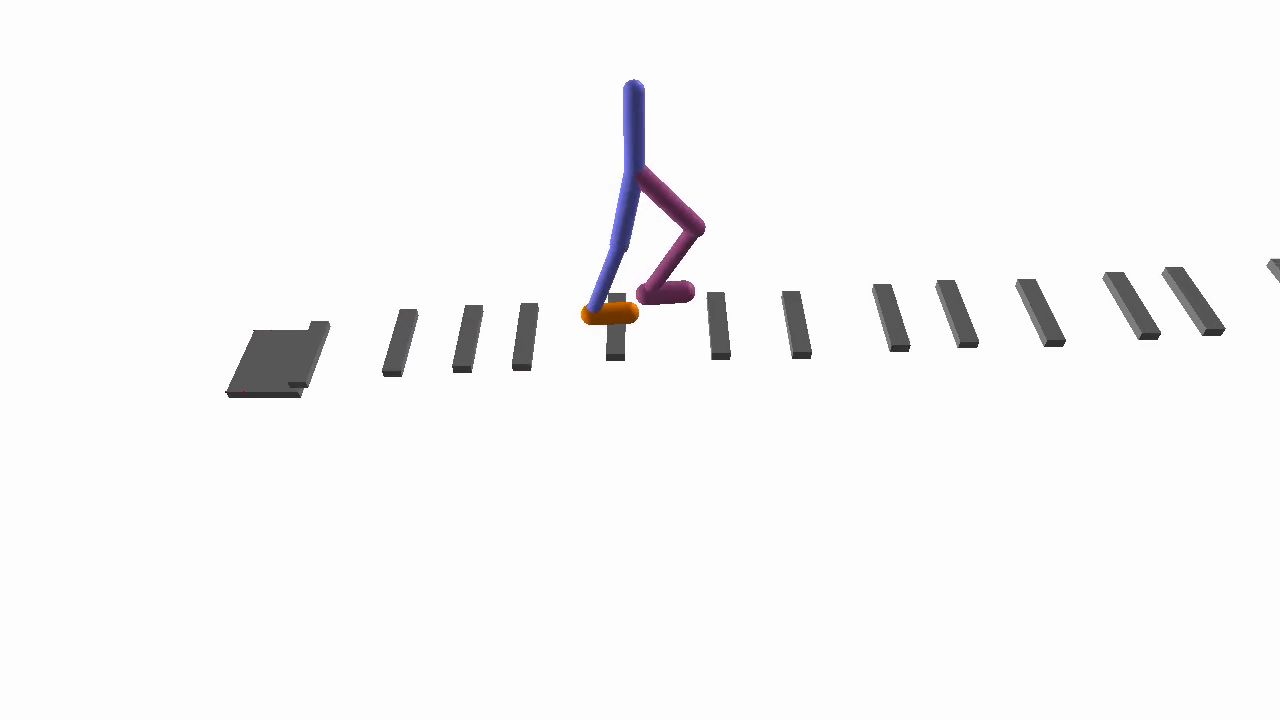
\includegraphics[width=0.48\textwidth]{../figures/2D_ep.png}
  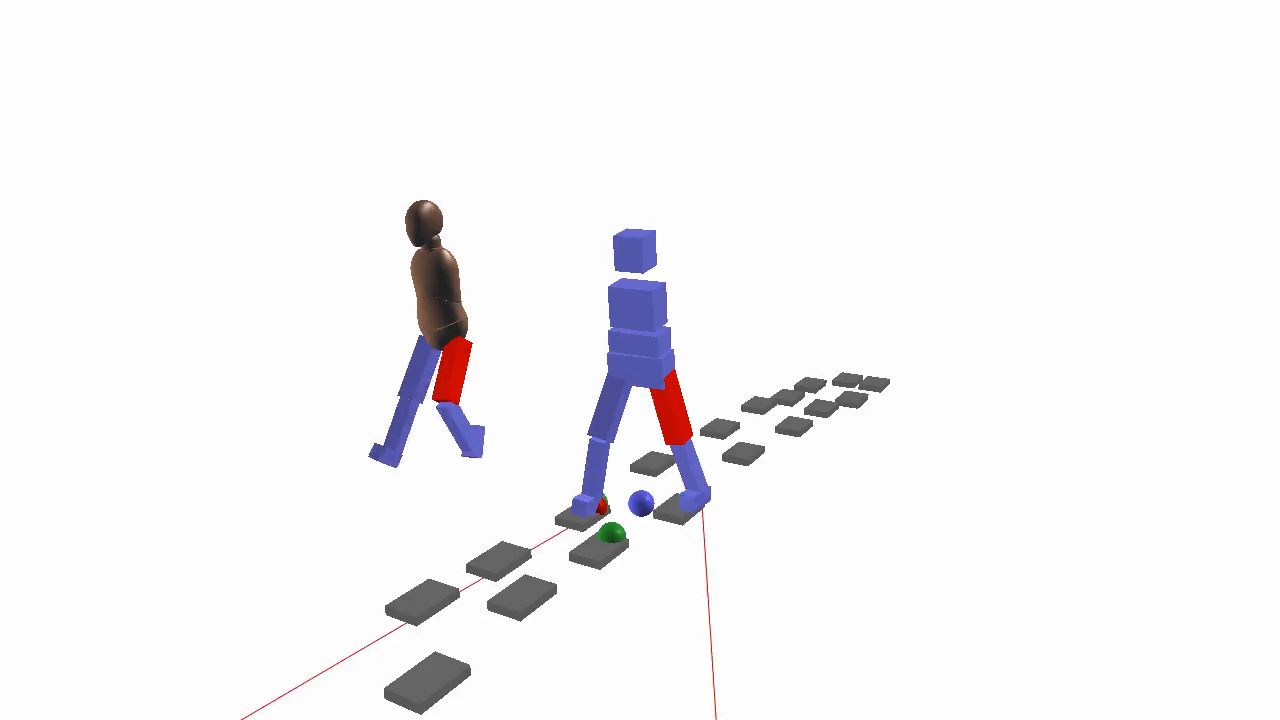
\includegraphics[width=0.48\textwidth]{../figures/3D_ep.png}
  \caption{Screenshots of example episodes.\label{fig:example episodes}}
\end{figure}

We evaluate CIM on the problem of dynamic biped locomotion over rough terrain.
Using the DART simulator \citep{lee2018dart}, we implement two RL problems as illustrated in Fig. \ref{fig:example episodes}.
In both environments, the goal is to walk across 16 stepping stones while maximizing the reward per step as defined in section \ref{sec:expert}.
Crashing terminates the episode early;
thus, the maximum reward per episode is 16.
The distribution of offsets between stepping stones is uniformly random.
In 2D, the offset in the X direction (the forward direction) is between 30 and 60 cm, while the Y offset (vertical) is between 5 and 10 cm.
In 3D, the X offset is 25--45cm, the Y offset is 0, and the Z offset is 30--50cm (alternating sign at each footstep).

Using the TG and learning algorithm described in Sec. \ref{sec:approach} above, our HLP is able to achieve reward $A\pm B$ (one standard deviation) after only $C$ simulated training footsteps.
\nhatch{Put actual numbers here.}
Examples of the final policies may be seen in the supplemental video.
To the best of our knowledge, our approach is the first to achieve such precise foot placement
using a fast, dynamic gait that requires no optimization during policy execution.

%Our secondary hypothesis is that the learned policy can be run in real-time while still achieving results comparable to more expensive, model-based optimization methods.
%This hypothesis is difficult to test, because model-based optimization methods are difficult to implement for direct comparison.
%Thus, our metric is simply the percent real time necessary to compute the control for the next time step, which we compare to numbers reported in optimization-based papers.

\subsection{Imitation learning ablations}

In this section, we evaluate CIM against a baseline that does not use imitation learning.
Instead, the baseline uses ARS \citep{mania2018simple} over entire episodes.
That is, at each iteration we update the HLP directly by estimating the gradient as a weighted combination of $Q$ random directions,
with weights determined by the change in total shaped reward as defined in section \ref{sec:expert}.
Note that this baseline is very similar to PMTG \citep{iscen2018pmtg}.
The only difference is that its policy architecture still uses the temporal abstraction explained in section \ref{sec:tg}.\footnote{
As we have not implemented a TG for biped locomotion that can be continuously modulated, this seems like the fairest comparison we could make.}

Based on a manual hyperparameter search, we decided that the baseline would use $Q=8$ random directions and a step size of $0.01$ decaying by $0.9$ at each iteration.
Furthermore, we decided that all $2Q$ rollouts during each iteration of ARS would use the same random seed (i.e. the same placement of stepping stones).
This reduces the variance of the gradient estimate in the sense that for this particular seed, the gradient estimate is more likely to be a good descent direction.
The random seed changes between iterations so that the learning algorithm gets to see the full distribution of testing environments.
Results were comparable or worse for the other hyperparameter settings that we tried.

For each approach (CIM and baseline) we run the experiment from scratch with four different starting random seeds.
Results on the 2D-Easy environment are shown in Fig. \ref{fig:ars baseline}.
The X axis shows the total number of simulated footsteps taken during training, and the Y axis shows total reward.
We plot the median and 10th/90th percentiles over 32 testing episodes (eight episodes for each of the four starting random seeds).

\begin{figure}
  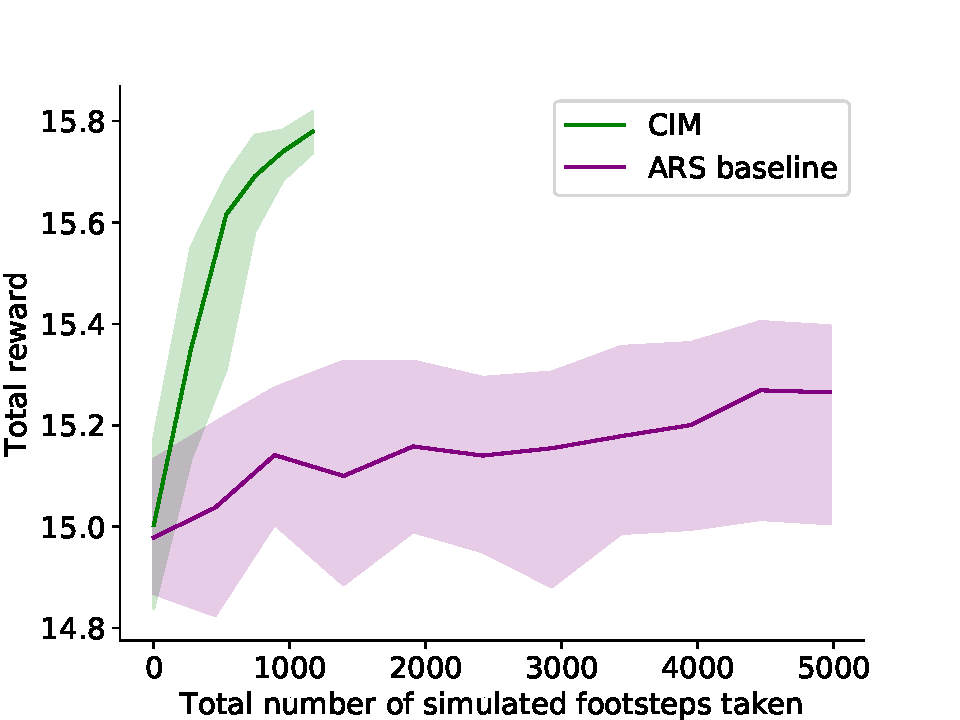
\includegraphics[width=0.48\textwidth]{../figures/ars_baseline.pdf}
  \caption{\label{fig:ars baseline} Training curves on 2D-Easy environment.}
\end{figure}

Taking advantage of simplifications to the credit assignment problem seems to be very helpful for this task.
Since the ARS baseline learns very slowly even on the 2D-Easy environment, we did not attempt to evaluate it on 2D-Hard.
In future work, to further validate the importance of imitation learning for periodic tasks, it would be interesting to compare CIM against a reinforcement learning algorithm such as PPO \citep{schulman2017proximal}.

\subsection{Curriculum learning ablations}

In this section, we evaluate CIM against a baseline that does not use curriculum learning.
Instead, the baseline begins training with a quadratic model in the final, most difficult testing environment.

Due to the sample complexity of the quadratic model, making this a fair comparison requires changing the training schedule used for imitation learning.
For the CIM experiments, we retrained the model every four rollouts,
but with a quadratic model this leads to disastrous overfitting and actually makes the expert \emph{worse}.
We tried several alternative imitation learning schedules.
Best results for the baseline were obtained by collecting an initial dataset of 32 rollouts and thereafter retraining every 16 rollouts.
Hyperparameters for the baseline were otherwise identical to the ones used for CIM.

Results on the 2D-Hard environment are shown in Fig. \ref{fig:nocur baseline}.
Like in Fig. \ref{fig:ars baseline},
we plot the median reward and 10th/90th percentiles over 32 testing episodes.

Even without a curriculum, the algorithm is able to find a policy that \emph{usually} achieves high reward.
However, CIM reaches the same median performance twice as quickly.
The story is similar for fifth-percentile performance.
\nhatch{TODO finish this once rerunning experiments finish}

\begin{figure}
  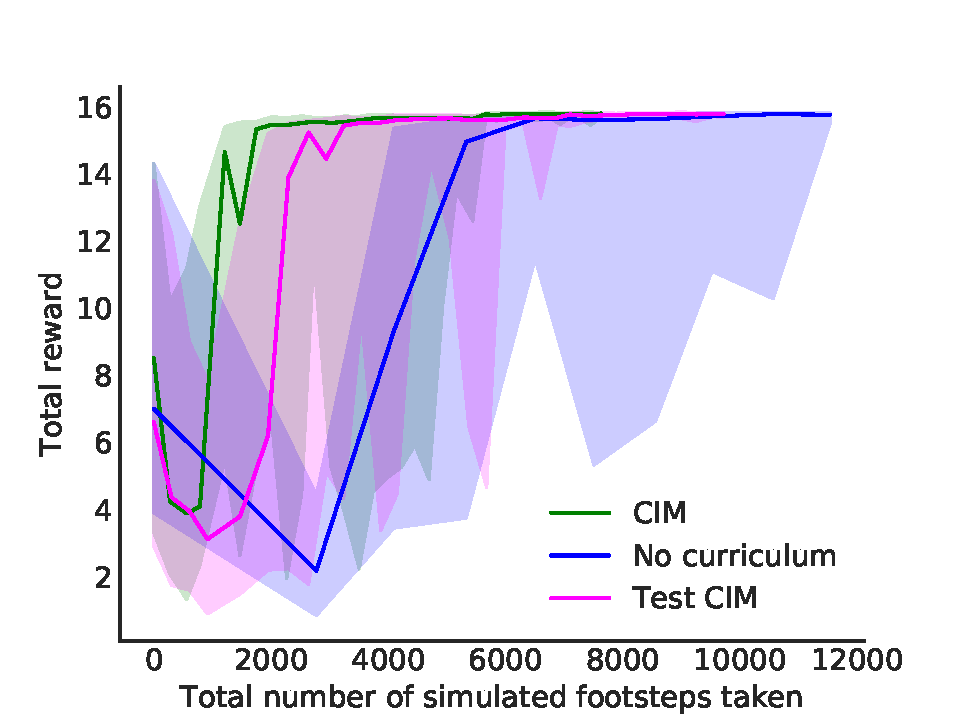
\includegraphics[width=0.48\textwidth]{../figures/nocur_baseline.pdf}
  \caption{\label{fig:nocur baseline} Training curves on 2D-Hard environment.}
\end{figure}

\section{Discussion}

Curricular imitative modulation is a general approach to integrating prior knowledge with machine learning in challenging, periodic robotic control problems.
Like PMTG \citep{iscen2018pmtg}, it simplifies the learning problem with the use of a well-designed trajectory generator.
Moreover, it further simplifies the learning problem by (1) using a temporally abstract high-level policy and (2) training with imitation and curriculum learning.

In particular, CIM is an intriguing direction for biped locomotion research.
To the best of our knowledge, our experiments are the first to achieve such precise foot placement
using a fast, dynamic gait that requires no optimization during policy execution.
However, one significant limitation of our work so far is that all experiments were performed in simulation.
In future work, we plan to investigate how to transfer policies trained with CIM to real-world bipedal robots.

\nhatch{future work: adaptive curriculum (adjusts to learner's current ability)}

Finally, we note that a significant portion of the effort for this project went into engineering the trajectory generator.
It might be possible to avoid this by training a trajectory generator using motion capture.
This would reduce the need for expert engineering and make it easier to test CIM on other robotic motion problems, such as manipulation.

%\section*{Acknowledgments}

\bibliographystyle{plainnat}
\bibliography{../bib}

\appendix

\section{Detailed description of trajectory generator for biped locomotion}

\label{app:simbicon}

\nhatch{TODO: list the exact inputs and outputs of the TG, in particular knowing the exact CoM is unnecessary}

In addition to the SIMBICON modifications discussed in Section \ref{sec:tg}, we also made the following changes:

\begin{enumerate}
  \item Set the target swing leg joint angles in the DOWN state using inverse kinematics (IK).
    Again, adjust the target swing heel location for the purposes of IK from the true target location based on the CoM speed and the same gain parameter as above.

  \item Control the swing ankle angle in world space to ensure that the swing heel is the first part of the foot to hit the ground.
    This does not have much effect on the step distance, but it helps make the dynamics of each impact more predictable, which is important for accurate function approximation.
    \nhatch{Again, all of this will have to be validated with ablations\dots.}

  \item In 3D, control the robot's heading using the stance hip.
    We found that setting the target stance hip angles using inverse kinematics and then using plain PD control was sufficient, without considering the effect of other torques on the stance hip.
\end{enumerate}

Note that there are also many additional parameters of SIMBICON that we could have exposed to the high-level policy; e.g. the stance ankle angle of the UP state.
Of course, we prefer to keep the problem dimension as low as possible, and we found that the short list of parameters given in Table \ref{table:params} was enough for our experiments.
We chose those parameters using a combination of intuition and trial-and-error.

\section{More details about the high-level policy}

It has the same input (``state'') as the basic controller: joint angles and velocities, stance heel location, and target step location (26 dimensions in 2D, 54 dimensions in 3D).
In addition, it sees the two previous target footstep locations.
(This is important in ``stepping stones'' environments where the exact location of the previous stepping stone might affect the dynamics.)
We exploit bilateral symmetry by mirroring the state and action if necessary so that the swing foot is always the right foot.

Because our dataset is relatively small, we use ridge regression to avoid overfitting.

\section{Detailed experimental setup}

All experiments are performed using the DART simulator at a simulation rate of 2000 Hz.
For now, we assume that perception is solved and that the step plan (in the form of a list of target step locations) is given by an oracle.\footnote{
In 3D, each target step location also includes a target \emph{heading}: the direction that the robot should face during the step.}
The problem is to choose motor torques to accomplish the given step plan.

Source code will be released upon publication.

\end{document}
